% !TEX encoding = UTF-8 Unicode

\section{\large Stock Return Series Prediction System}

%%%%%%%%%%%%%%%%%%%%

\subsection{System Overview}

\begin{frame}[fragile,t]{System Overview}
	\begin{figure}[!hbt]
    \center
    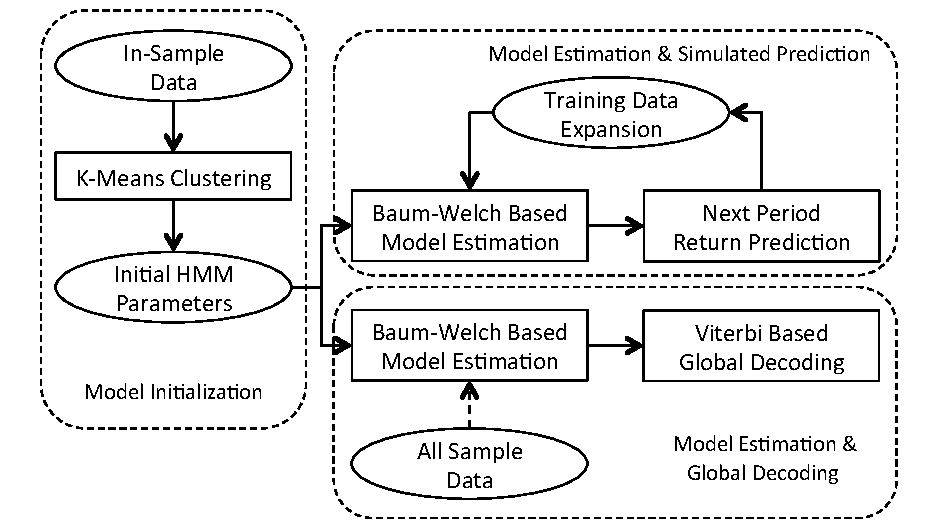
\includegraphics[width=0.85\textwidth]{system.pdf}
    \caption{Overview of the stock return series prediction system}
    \label{fig:system:overview}
    \end{figure}
\end{frame}

%%%%%%%%%%%%%%%%%%%%

\subsection{Model Initialization}

\begin{frame}[fragile,t]{Model Initialization}
	\begin{figure}[!hbt]
    \center
    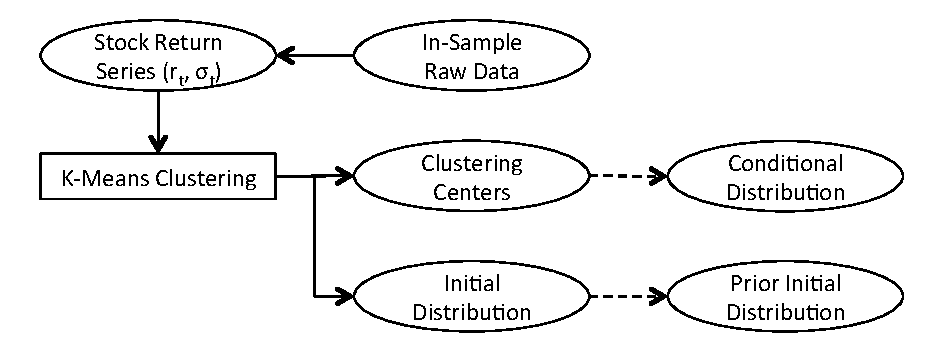
\includegraphics[width=0.8\textwidth]{initialization.pdf}
    \caption{Model initialization module}
    \label{fig:system:init}
    \end{figure}

    \begin{itemize}
    \item Transform the raw data into specified data structure (data tidying).
    \item Pre-process the raw data for observed variable series as K-Means input.
    \end{itemize}
\end{frame}

%%%%%%%%%%%%%%%%%%%%

\subsection{Simulated Prediction}

\begin{frame}[fragile,t]{EM-Based Model Estimation}
	\begin{figure}[!hbt]
    \center
    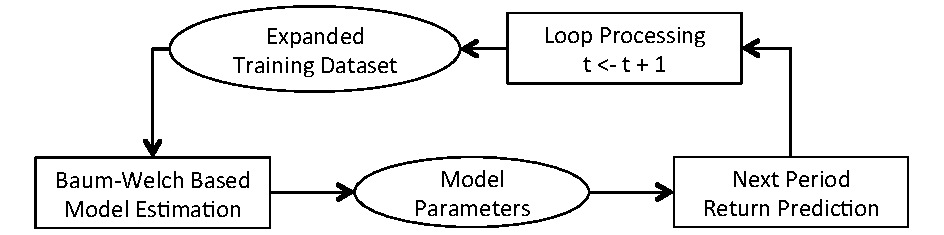
\includegraphics[width=0.8\textwidth]{EM.pdf}
    \caption{EM based model estimation procedure}
    \label{fig:system:EM}
    \end{figure}

    \begin{itemize}
    \item Carry out model estimation with EM algorithm (Baum-Welch).
    \item Calibrated parameters: hidden states initial distribution $\bpi$, 
    	hidden states final distribution $\bdelta$,
    	state transition matrix $\bGamma$, 
    	conditional distribution parameters $(\bmu,\bsigma)$.
    \item The model estimation procedure is \textit{adaptive}, 
    	i.e.\,it incorporates the new historical return information when the loop processes.
    \end{itemize}
\end{frame}

\begin{frame}[fragile,t]{Prediction}
    \begin{itemize}
    \item Two different ways to predict the \textit{price} of the next period:
    	\[ \begin{aligned}
		\text{static:}\ \hat{P}_t & = P_0 e^{\sum_{i=1}^{t}\hat{r}_i}, \\
		\text{adaptive:}\ \hat{P}_t & = P_{t-1} e^{\hat{r}_t},
		\end{aligned} \]
		where $P_{t-1}$ is the real price at time $t-1$ and 
		$P_0$ is the price of the first day when the prediction procedure begins.
    \item The first prediction procedure only considers the information of the returns, 
    	and thus the errors of predictions accumulate and are reflected on the predicted price.
    \item The second (so-called \alert{adaptive prediction}) procedure considers both the return and 
    	the \textit{price level} at $t-1$ to predict the price at $t$.
    \end{itemize}
\end{frame}

%%%%%%%%%%%%%%%%%%%%

\subsection{Global Decoding}

\begin{frame}[fragile,t]{Global Decoding}
	\begin{figure}[!hbt]
    \center
    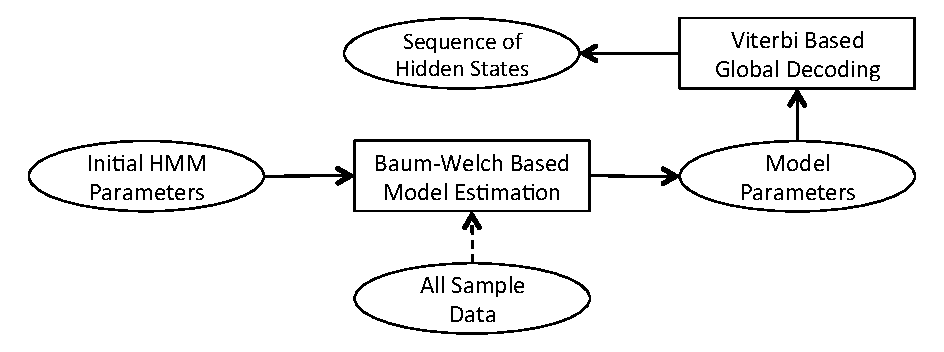
\includegraphics[width=0.8\textwidth]{decoding.pdf}
    \caption{Global decoding module}
    \label{fig:system:decoding}
    \end{figure}

    \begin{itemize}
    \item Independent with the simulated prediction module.
    \item Conduct Viterbi algorithm based global decoding to 
    	deduce the most probable sequence of hidden states during the observation period.
    \end{itemize}
\end{frame}